\section{DataModel (Data Access Layer)}\label{sec:datamodel}
The DataModel module is the business logic core of this application.
Inside this module there is the implementation of the Object Document Mapping
(ODM) that has been realized specifically for our application.
Instead of using base classes provided by the MongoDB connector such as Document
and Bson classes, we developed a POJO mapping exploiting the possibility that
MongoDB Java Connector give us, to automatically convert a Document from the
Database to a Plain old Java Object. The clear advantages of this approach are
that we don't have to pick every field of a document manually, enforcing OOP
typical features, like encapsulation, and improving code reusability. On the
other hand the objects retrieved from the DB don't have any "history tracking"
on the operation performed on them outside the database, so what we had to do
is to develop from scratch a CRUD operation tracking on each object, and a way
to resolve the tracking of the operations performed, in a MongoDB CRUD
operation.
Our solution is based on the intensive usage of Reflection APIs, to track the
operations performed on objects outside the database, and a series of
PojoManagers, that have to know how to threat a Pojo when it's stored in the
database.
This Manager-based approach is inspired to the work done from spreadly used libraries such
as Hibernate (for SQL databases) or Mongoose, for javascript.
Even if the designing phase of this approach is far more tricky and complicated
then using Document and Bson classes, we have a considerably valuable ease when
dealing with the database, from the application. In this way we can easily build 
programmatically dynamic aggregation pipelines, and simple CRUD operations can
be done with fewer code lines.

\begin{landscape}
	\begin{figure}[!h]
		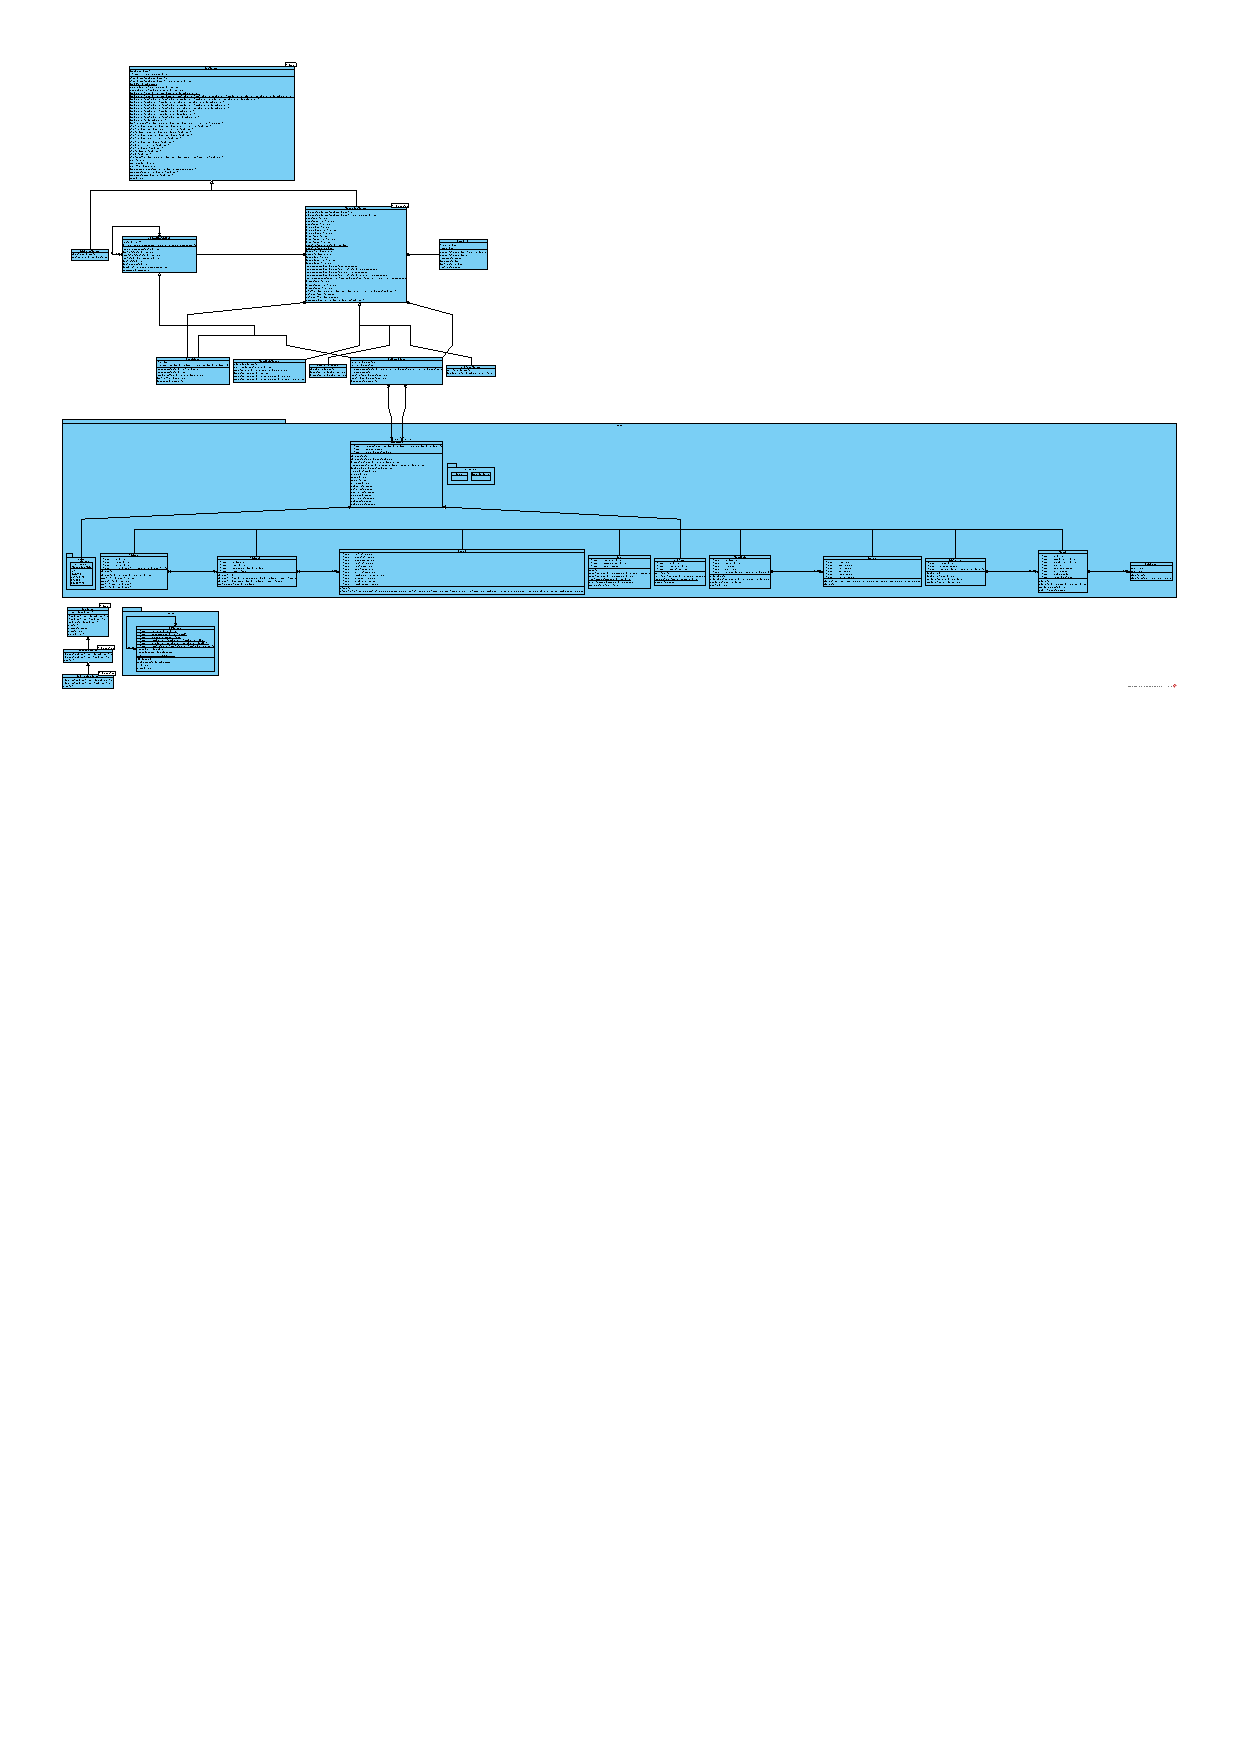
\includegraphics{app.datamodel}
		\caption*{\textbf{Figure~\ref{fig:datamodel}}}
		\captionlistentry{}\label{fig:datamodel}
	\end{figure}
\end{landscape}
